\documentclass{beamer}
\usepackage{graphicx}
\usepackage{paralist}
\usepackage{outlines}

\title{Week 6 Outline}
\author{Mendocino College - Digital Image Manipulation with Photoshop}
\titlegraphic{\vspace{-10mm}
\includegraphics[width = .9\textwidth]{images/photoshop.jpg}} 
\date{\vspace{-5em}} 


\mode <presentation>
\usetheme{Warsaw}
\usecolortheme{default}

\setbeamerfont{footline}{size=\fontsize{5}{8}\selectfont}

\definecolor{darkred}{rgb}{20,0,0}
\definecolor{darkgreen}{RGB}{40,110,20}
\definecolor{darkpurple}{RGB}{30,0,30}
\definecolor{chardonnay}{RGB}{255, 255, 204}

\setbeamercolor*{palette primary}{fg=white, bg=darkgreen}


\begin{document}
	{
		\setbeamertemplate{footline}{} 
		\setbeamertemplate{headline}{} 
		\begin{frame}
			\vspace{-35pt}
			\maketitle
		\end{frame}
	}

		\section{Announcements}
			\subsection{Syllabus Update}		
			\begin{frame}
				\frametitle{Syllabus Update}
				\begin{columns}
					\column{.6\textwidth}
					\begin{outline}
						\1 Not everyone has access to canvas, so we cannot shift lectures online.
						\1 Lecture Quizes have been removed.
						\1 Discussions were worth 20\%, and are now worth a total of 15\%.
						\1 Weekly Assignments are now Weekly Exercises.
						\1 Weekly Exercises have from from 20\% to 15\%.
						\1 Assignments are now individual mini-projects, worth 10\% of your total grade.
					\end{outline}
					\column{.5\textwidth}
					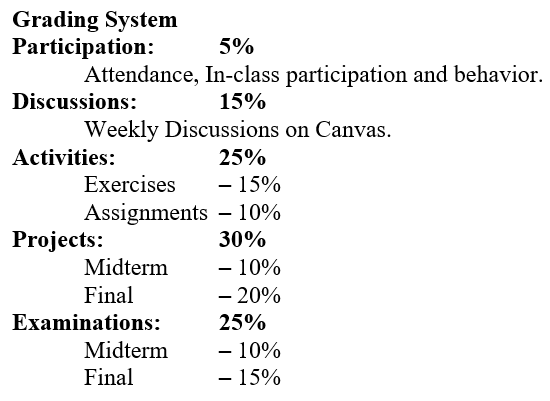
\includegraphics[width=1.0\textwidth]{images/grading system update.png}
				\end{columns}
			\end{frame}


	\section{Lecture Topics}
			\subsection{Lecture Topics}		
	\begin{frame}
		\frametitle{Lecture Topics for Week 6}
				\begin{outline}
					\1 Masks
					\1 Smooth and Feathering Edges
					\1 Paint Bucket and Gradient Tools
					\1 Resolution
					\1 Borders
				\end{outline}
		\end{frame}

			\subsection{Masks}		
				\begin{frame}
					\frametitle{Masks}
					\begin{outline}
						\1 Masks
						\1 Layer Masks
						\1 Select and Mask
						\1 Quick Mask
					\end{outline}
				\end{frame}
	
			\subsection{Smooth and Feathering Edges}		
				\begin{frame}
					\frametitle{Smooth and Feathering Edges}
						\begin{outline}
							\1 Feathering Edges
							\1 Smoothing Edges
							\1 Blurring Edges
						\end{outline}
				\end{frame}
			
			\subsection{Gradient and Paint Bucket Tools}		
				\begin{frame}
					\frametitle{Gradient and Paint Bucket Tools}
					\begin{outline}
						\1 Gradient Tool
						\1 Gradient Editor
						\1 Paint Bucket Tool
					\end{outline}
				\end{frame}
			
		\subsection{Resolution and Borders}		
			\begin{frame}
				\frametitle{Resolution and Borders}
				\begin{outline}
					\1 Resolution
					\1 Pixels Per Inch
					\1 Image Size
					\1 Canvas Size
					\1 Borders
				\end{outline}
			\end{frame}
			
		\section{Assignments}
			\subsection{Weekly Exercises}		
			\begin{frame}
				\frametitle{Exercises for Week 6}
				\begin{outline}
					\1 Masks
					\1 Feathering
					\1 Gradient Tool
					\1 Paint Bucket and Border
				\end{outline}
			\end{frame}
		
		\subsection{Assignment}		
			\begin{frame}
				\frametitle{Assignment \#3}
				\begin{outline}
					\1 Paint your own Picture!
					\1 Start with a blank image and use all the tools we have learned so far to create your very digital image!
					\1 You cannot import any images, and must create your final image completely from scratch.
					\1 Your final composition must have at least 7 distinct and different layers.  
				\end{outline}
			\begin{center}
			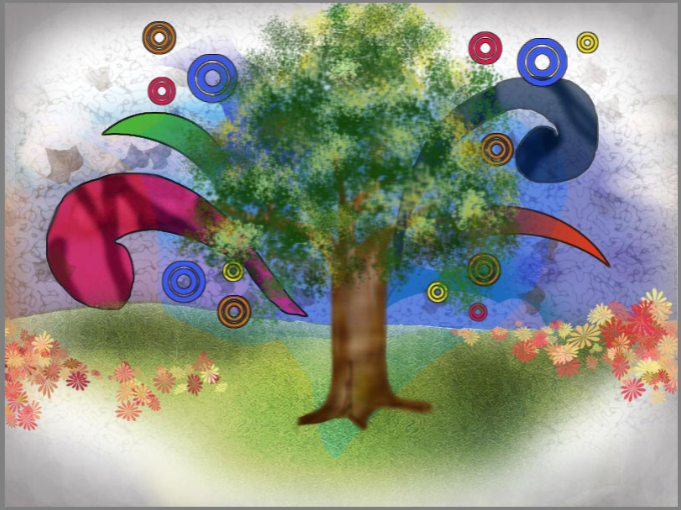
\includegraphics[width=0.6\textwidth]{images/paint picture assignment.png}
			\end{center}
			\end{frame}
	
			\subsection{Discussion}		
				\begin{frame}
					\frametitle{Videos \& Articles for Discussion Post}
					\begin{outline}
						\1 YouTube Video:  PPI is Imaginary! PPI vs DPI vs Resolution
							\2 By:  PiXimperfect
							\2 Duration:  14 minutes and 29 seconds
						\1 YouTube Video:  PHOTOSHOP: Beginner’s Guide to Masking 2022
							\2 By:  tutvid
							\2 Duration:  18 minutes and 41 seconds
					\end{outline}
					
				\end{frame}

				\begin{frame}
					\frametitle{Research Topics for Discussion Post}
					\begin{columns}
						\column{.5\textwidth}
						\begin{outline}
							\1 Layer Masks
							\1 Quick Masks
							\1 Select and Mask
							\1 Gradient Tool
							\1 Paint Bucket Tool
							\1 Feathering
							\1 Smoothing
						\end{outline}
						\column{.5\textwidth}
					\begin{outline}
						\1 Google Drive
						\1 Foreground \& Background Colors
						\1 Canvas Size
						\1 Image Size
						\1 Resolution
						\1 PPI (Pixels Per Inch)
					\end{outline}
					\end{columns}
				\end{frame}
	
	\section{}	
		\subsection{End Card}
		\begin{frame}
			\frametitle{End Card}	
			\begin{columns}
				\column{.6\textwidth}
				\vspace{-25pt}
				\begin{itemize}
					\item Joshua Paul Barnard
					\item Computer Science Instructor
					\item Mendocino College
				\end{itemize}
			\space
				\begin{itemize}
					\item Presentation was made in \LaTeX
					\item For the Fall 2022 semester.  
				\end{itemize}
				\begin{itemize}
					\item jbarnard@mendocino.edu
					\item github.com/JoshuaPaulBarnard
				\end{itemize}
				\column{.45\textwidth}
				
\includegraphics[width=.85\textwidth]{images/shone farm wine pouring - vert.png}
			\end{columns}
		\end{frame}
	
\end{document}